\chapter{绪论}

这是 \zjuthesis 的示例文档。格式样列很大一部分是直接从薛瑞尼的 \thuthesis\footnote{《清华大学学位论文 \LaTeX 模板》,\url{http://thuthesis.sourceforge.net/}} 示例文档中拿来的,因为 \thuthesis 的示例很全面,我懒得再重新发明轮子。具体如何使用这份模板,还是要看《\zjuthesis 使用说明》。

\section{字体示例}

九齿钉耙学名{\kaiti 上宝沁晶耙},是俺的武器。九齿钉耙并非普通的农具,而是由太上老君\footnote{太上老君,三清之第三位。又称“道德天尊”、“混元老君”、“降生天尊”、“太清大帝”等。}用神冰铁亲自锤炼,借五方五帝、六丁六甲之力锻造而成,有诗为证:
\nomenclature{上宝沁晶耙}{猪八戒的武器,是由太上老君锤炼的农具。}

\vspace{-5mm}

\begin{tabbing}
\hspace{20mm} \= \hspace{20mm} \= \hspace{80mm} \kill\\
 \> 字体      \>  \hspace{26mm} 示例 \\
 \> fangsong \> \fangsong 老君自己动钤锤,荧惑亲身添炭屑。 \\
 \>          \> \fangsong 五方五帝用心机,六丁六甲费周折。 \\
 \>          \> \fangsong 造成九齿玉垂牙,铸就双环金坠叶。 \\
 \> heiti    \> \heiti 身妆六曜排五星,体按四时依八节。 \\
 \>          \> \heiti 短长上下定乾坤,左右阴阳分日月。 \\
 \>          \> \heiti 六爻神将按天条,八卦星辰依斗列。 \\
 \> kaiti    \> \kaiti 名为上宝沁金钯,进与玉皇镇丹阙。 \\
 \>          \> \kaiti 因我修成大罗仙,为吾养就长生客。 \\
 \>          \> \kaiti 敕封元帅号天蓬,钦赐钉钯为御节。 \\
 \> lishu    \> \lishu 举起烈焰并毫光,落下猛风飘瑞雪。 \\
 \>          \> \lishu 天曹神将尽皆惊,地府阎罗心胆怯。 \\
 \>          \> \lishu 人间那有这般兵,世上更无此等铁。 \\
 \> songti   \> \songti 随身变化可心怀,任意翻腾依口诀。 \\
 \>          \> \songti 相携数载未曾离,伴我几年无日别。 \\
 \>          \> \songti 日食三餐并不丢,夜眠一宿浑无撇。 \\
 \> youti    \> \youti 也曾佩去赴蟠桃,也曾带他朝帝阙。 \\
 \>          \> \youti 皆因仗酒却行凶,只为倚强便撒泼。 \\
 \>          \> \youti 上天贬我降凡尘,下世尽我作罪孽。 \\
 \> default  \> 石洞心邪曾吃人,高庄情喜婚姻结。 \\
 \>          \> 这钯下海掀翻龙鼍窝,上山抓碎虎狼穴。 \\
 \>          \> 诸般兵刃且休题,惟有吾当钯最切。 \\
 \>          \> 相持取胜有何难,赌斗求功不用说。 \\
 \>          \> 何怕你铜头铁脑一身钢,钯到魂消神气泄!
\end{tabbing}

\section{各种示例}

\zjubiaozhun 没有规定英文字体,\zjuthesis 将中、英文统一设置为仿宋。

当存在连续多个表格、图片时,\LaTeX 的排版效果不佳,所以这里不时插播些王勃的《腾王阁序》,有空的话也看两眼。

《腾王阁序》第一段:豫章故郡,洪都新府。星分翼轸,地接衡庐。襟三江而带五湖,控蛮荆而引瓯越。物华天宝,龙光射牛斗之墟;人杰地灵,徐孺下陈蕃之榻。雄州雾列,俊采星驰。台隍枕夷夏之交,宾主尽东南之美。都督阎公之雅望,棨戟遥临;宇文新州之懿范,襜帷暂驻。十旬休假,胜友如云;千里逢迎,高朋满座。腾蛟起凤,孟学士之词宗;紫电青霜,王将军之武库。家君作宰,路出名区,童子何知,躬逢胜饯。

《腾王阁序》第二段:时维九月,序属三秋。潦水尽而寒潭清,烟光凝而暮山紫。俨骖騑于上路,访风景于崇阿。临帝子之长洲,得天人之旧馆。层台耸翠,上出重霄;飞阁翔丹,下临无地。鹤汀凫渚,穷岛屿之萦回;桂殿兰宫,即冈峦之体势。披绣闼,俯雕甍:山原旷其盈视,川泽纡其骇瞩。闾阎扑地,钟鸣鼎食之家;舸舰迷津,青雀黄龙之轴。云销雨霁,彩彻区明。落霞与孤鹜齐飞,秋水共长天一色。渔舟唱晚,响穷彭蠡之滨;雁阵惊寒,声断衡阳之浦。

\subsection{图片示例}

附上照片一张,来源 Wikipedia。

\begin{figure}[htbp]
  \centering
  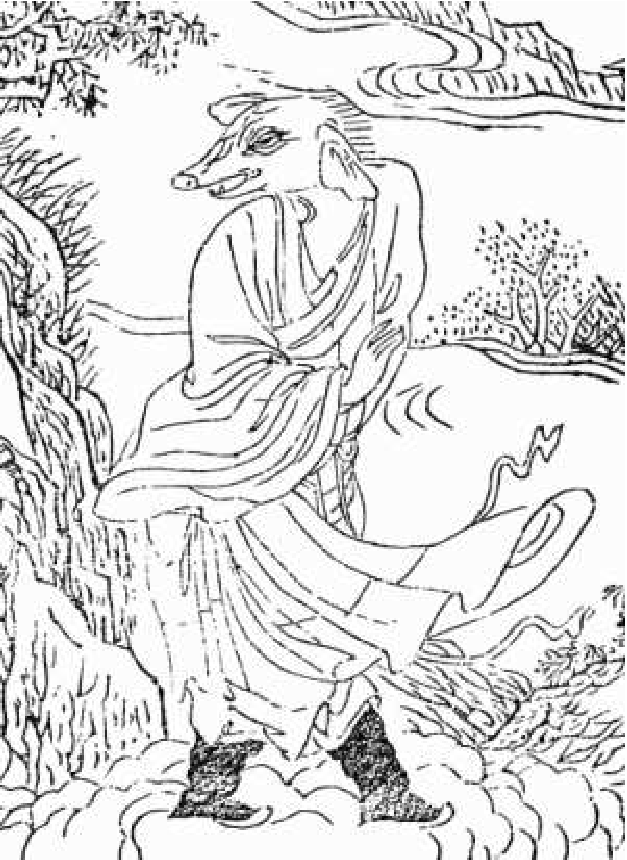
\includegraphics[scale=0.8]{images/zhubajie.pdf}
  \caption{玉照}
  \label{fig:example}
\end{figure}
\nomenclature{玉照}{玉做的照片,通常会令人联想到浴照。}

这里用的是 EPS 图,我只使用 dvips,所以 pdflatex 对 PNG 的支持情况如何不得而知。\zjuthesis 也附带了一张 PNG 格式的玉照,你可以试试看如何。

\subsection{表格示例}

我自己的论文表格量很大,模板照搬我的论文的设置,表格相关的宏包加了很多,具体见《\zjuthesis 使用说明》。

先看一个简单表格 \ref{tab:simple-table}:

\begin{table}[htb]
  \centering
  \caption{模板中的表格宏包}
  \label{tab:simple-table}
    \begin{tabular}{ll}
      \toprule
      \multicolumn{1}{m{20mm}}{\heiti\centering 宏包} & \multicolumn{1}{m{80mm}}{\heiti\centering 描述} \\
      \midrule
      longtable & 绘制跨页的表格。 \\
      booktabs & 三线表中的那三条线的命令来自这里。\\
      caption2 & 用于设置标题很方便,已经 obsolated,不过 \TeX Live 中还有。\\
      multirow & 跨行的单元格用这个宏包。\\
      dcolumn  & 想让表格小数点对齐吗?用这个宏包吧。\\
      \rowcolor[gray]{.9} colortbl & 表格上色。自己看着爽而已,打印出来都是黑白的。 \\
      threeparttable & 用来给表格添加脚注啥的很方便。 \\
      array & 忘了用来做什么了,但似乎很重要。 \\
      \bottomrule
    \end{tabular}
\end{table}

再来看个复杂的表格 \ref{tab:complex-table}。本想像 \thuthesis 那样示例一下表格内画斜线的功能,但失败了,所以建议不要用这种画斜线的表格。另外,threeparttable 在处理标题和脚注的距离时有些异常,能不用就不要用了。

\begin{center}
\vspace{-6mm}
\begin{threeparttable}
  \caption{复杂的表格}
  \label{tab:complex-table}
  \begin{tabular}{l....}
    & & & & \\[-8mm]
    \toprule
     \multirow{2}*{} 
           & \multicolumn{2}{c}{First Half} & \multicolumn{2}{c}{Second Half}\\\cline{2-5}
               & \multicolumn{1}{l}{1st Qtr} & \multicolumn{1}{l}{2nd Qtr} 
               & \multicolumn{1}{l}{3rd Qtr} & \multicolumn{1}{l}{4th Qtr} \\
    \midrule
      East$^{*}$ &   20.4&   7.4&   90&     20.4 \\
      West$^{**}$ &   30.6 &  338.6 &   34.6 &  31.6 \\
    \bottomrule
  \end{tabular}
  \vspace{-9mm}
  \begin{tablenotes}[para]
    \footnotesize 注:数据来源《\thuthesis 使用手册》。
  \end{tablenotes}
\end{threeparttable}
\vspace{5mm}
\end{center}

《腾王阁序》第三段:遥襟甫畅,逸兴遄飞。爽籁发而清风生,纤歌凝而白云遏。睢园绿竹,气凌彭泽之樽;邺水朱华,光照临川之笔。四美具,二难并。穷睇眄于中天,极娱游于暇日。天高地迥,觉宇宙之无穷;兴尽悲来,识盈虚之有数。望长安于日下,目吴会于云间。地势极而南溟深,天柱高而北辰远。关山难越,谁悲失路之人;沟水相逢,尽是他乡之客。怀帝阍而不见,奉宣室以何年。嗟乎!时运不齐,命途多舛;冯唐易老,李广难封。屈贾谊于长沙,非无圣主;窜梁鸿于海曲,岂乏明时。所赖君子见机,达人知命。老当益壮,宁移白首之心;穷且益坚,不坠青云之志。酌贪泉而觉爽,处涸辙而相欢。北海虽赊,扶摇可接;东隅已逝,桑榆非晚。孟尝高洁,空余报国之情;阮籍猖狂,岂效穷途之哭!

《腾王阁序》第四段:勃,三尺微命,一介书生。无路请缨,等终军之弱冠;有怀投笔,爱宗悫之长风。舍簪笏于百龄,奉晨昏于万里。非谢家之宝树,接孟氏之芳邻。他日趋庭,叨陪鲤对;今兹捧袂,喜托龙门。杨意不逢,抚凌云而自惜;钟期相遇,奏流水以何惭。呜呼!胜地不常,盛筵难再;兰亭已矣,梓泽丘墟。临别赠言,幸承恩于伟饯;登高作赋,是所望于群公。敢竭鄙怀,恭疏短引;一言均赋,四韵俱成。请洒潘江,各倾陆海云尔。 

\subsection{定理示例}

\thuthesis 定义了很多定理格式,下面都是从 \thuthesis 搬来的例子。我自己只用到了“假设”,对于公式、证明之类的格式完全无知,你如有其他需要可以在 88 \TeX 版上提出来,我再添加。

{\youti 照搬部分开始:}

\begin{hypo}
待月西厢下,迎风户半开;隔墙花影动,疑是玉人来。
\begin{eqnarray}
  \label{eq:eqnxmp}
  c & = & a^2 - b^2\\
    & = & (a+b)(a-b)
\end{eqnarray}
\end{hypo}

\begin{defin}
子曰:「道千乘之国,敬事而信,节用而爱人,使民以时。」
\end{defin}

\begin{theo}
犯我强汉者,虽远必诛。\hfill —— 陈汤(汉)
\end{theo}

\begin{pro}
天不言自高,水不言自流。
\begin{gather*}
\begin{split} 
\varphi(x,z)
&=z-\gamma_{10}x-\gamma_{mn}x^mz^n\\
&=z-Mr^{-1}x-Mr^{-(m+n)}x^mz^n
\end{split}\\[6pt]
\begin{align} \zeta^0&=(\xi^0)^2,\\
\zeta^1 &=\xi^0\xi^1,\\
\zeta^2 &=(\xi^1)^2,
\end{align}
\end{gather*}
\end{pro}

{\youti 照搬部分结束。}

\subsection{公式示例}

我公式用非常少,所以公式的情况并不了解,这部分示例也完全照搬 \thuthesis。如果有什么问题或要求,可以贴到 88 \TeX 版。
\nomenclature{$\chi^2$}{卡方}

{\youti 照搬部分开始:}

贝叶斯公式如式 (\ref{equ:chap1:bayes}),其中 $p(y|\mathbf{x})$ 为后验;$p(\mathbf{x})$ 为先验;分母 $p(\mathbf{x})$ 为归一化因子。

\begin{equation}
\label{equ:chap1:bayes}
p(y|\mathbf{x}) = \frac{p(\mathbf{x},y)}{p(\mathbf{x})}=
\frac{p(\mathbf{x}|y)p(y)}{p(\mathbf{x})} 
\end{equation}

论文里面公式越多,\TeX 就越 happy。再看一个 \textsf{amsmath} 的例子:

\newcommand{\envert}[1]{\left\lvert#1\right\rvert} 

\begin{equation}\label{detK2}
\det\mathbf{K}(t=1,t_1,\dots,t_n)=\sum_{I\in\mathbf{n}}(-1)^{\envert{I}}
\prod_{i\in I}t_i\prod_{j\in I}(D_j+\lambda_jt_j)\det\mathbf{A}
^{(\lambda)}(\overline{I}|\overline{I})=0.
\end{equation} 

大家在写公式的时候一定要好好看 \textsf{amsmath} 的文档,并参考模板中的用法:

\begin{multline*}\tag{[b]} % 这个出现在索引中的
\int_a^b\biggl\{\int_a^b[f(x)^2g(y)^2+f(y)^2g(x)^2]
 -2f(x)g(x)f(y)g(y)\,dx\biggr\}\,dy \\
 =\int_a^b\biggl\{g(y)^2\int_a^bf^2+f(y)^2
  \int_a^b g^2-2f(y)g(y)\int_a^b fg\biggr\}\,dy
\end{multline*}

其实还可以看看这个多级规划:

\begin{equation}\label{bilevel}
\left\{\begin{array}{l}
\max\limits_{{\mbox{\footnotesize\boldmath $x$}}} F(x,y_1^*,y_2^*,\cdots,y_m^*)\\[0.2cm]
\mbox{subject to:}\\[0.1cm]
\qquad G(x)\le 0\\[0.1cm]
\qquad(y_1^*,y_2^*,\cdots,y_m^*)\mbox{ solves problems }(i=1,2,\cdots,m)\\[0.1cm]
\qquad\left\{\begin{array}{l}
    \max\limits_{{\mbox{\footnotesize\boldmath $y_i$}}}f_i(x,y_1,y_2,\cdots,y_m)\\[0.2cm]
    \mbox{subject to:}\\[0.1cm]
    \qquad g_i(x,y_1,y_2,\cdots,y_m)\le 0.
    \end{array}\right.
\end{array}\right.
\end{equation}

{\youti 照搬部分结束。}

\subsection{参考文献}

参考文献建议使用 BiB\TeX,bibitem 方式我虽然听说过,但没尝试过。

参考文献的例子:书籍文献\citez{tex,companion};杂志文章,单独的\citez{article1},并列的\citez{article2,article3},合并的\citez{article1,article2,article3};硕士论文\citez{master},俺的旧文一篇;博士论文\citez{doctor},沙师弟的大作;论文集或 Handbook\citez{collection},会议论文集\citez{proceeding},会议论文\citez{conference};带页码脚标的\citez[123]{tex}。

% 参考文献的例子(作者在括号内):书籍文献\citezp{tex,companion};杂志文章\citezp{article1};硕士论文\citezp{master},俺的旧文一篇;博士论文\citezp{doctor},沙师弟的大作;论文集或Handbook\citezp{collection},会议论文集\citezp{proceeding},会议论文\citezp{conference};带页码脚标的\citezp[123]{tex}。

% 参考文献的例子(作者在括号外):书籍文献~\citezt{tex,companion};杂志文章~\citezt{article1};硕士论文~\citezt{master};博士论文~\citezt{doctor};论文集或~Handbook~\citezt{collection},会议论文集~\citezt{proceeding},会议论文~\citezt{conference},带页码脚标的~\citezt[123]{tex}。

